
\subsection{Prof.\ Dr.\ rer. nat. Holger Karl}
%\noindent\textbf{\large Prof.\ Dr.\ rer. nat. Holger Karl} ~geboren am ????, männlich \\
\begin{minipage}{11cm}
\begin{tabular}{@{}l@{\qquad}l}
geboren am 15.02.1970, männlich                          & \\
Universit\"at Paderborn                            & \\
Institut f\"ur Informatik                          & \\
Warburger Straße 100                               & \\
33098 Paderborn                                    & \\
Telefon: (05251) 60-5375                           & \\
Fax: (05251) 60-5377                               & \\
E-Mail: holger.karl@upb.de                                       & \\
\href{https://cs.uni-paderborn.de/cn/team/staff/karl/}{https://cs.uni-paderborn.de/cn/team/staff/karl/}     & \\
C4 Professor für Rechnernetze                              &
\end{tabular}
\end{minipage} \hfill
\begin{minipage}{3.5cm}
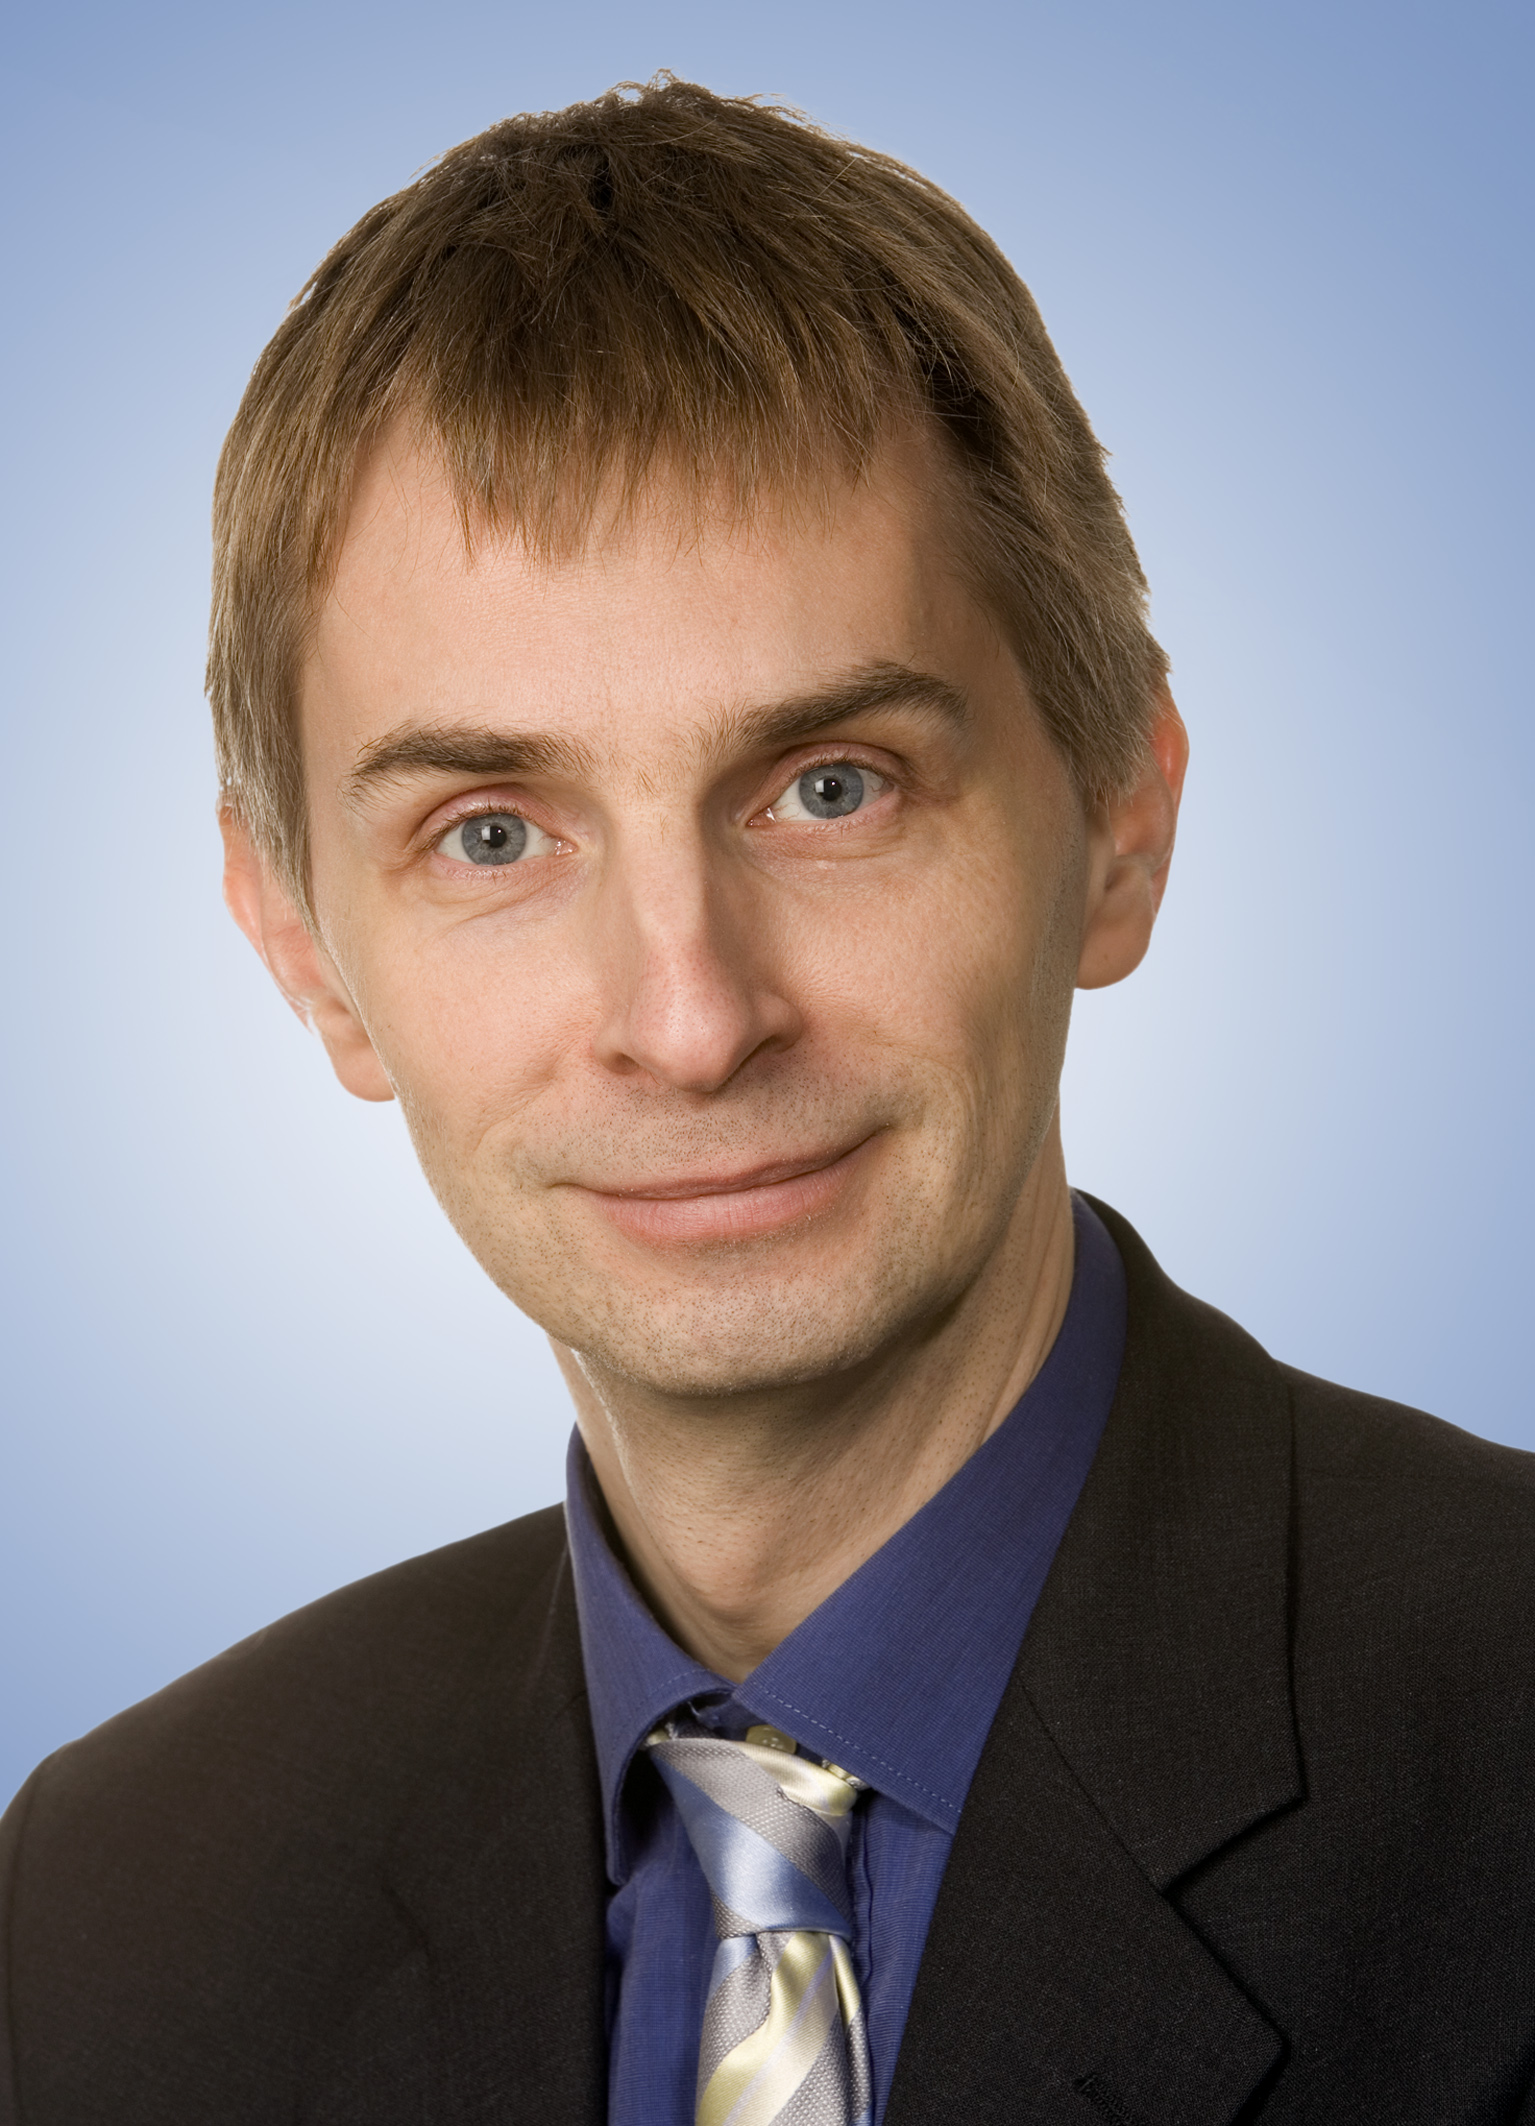
\includegraphics[width=3.5cm]{figures/signatures/Karl.jpg}
\end{minipage}


\vspace{0.9em}
\noindent\textsc{\textbf{Akademische Ausbildung mit Abschluss}}
%\headspace

Studium der Informatik, 10/1990 - 07/1996, Universität Karlsruhe \\
Abschluss: Diplom; Betreuer der Diplomarbeit: Prof.~Dr.~Theo Ungerer


\vspace{0.9em}
\noindent\textsc{\textbf{Wissenschaftliche Abschlüsse}}
%\headspace

Promotion: Informatik, Humboldt-Universität zu Berlin, 1999 \\
Betreuer: Prof.\ Dr.\ Miroslav Malek

\vspace{0.9em}
\noindent\textsc{\textbf{Beruflicher Werdegang ab Studienabschluss}}
%\headspace

seit 10/2004, Professor (C4), Universität Paderborn \\
01/2000 - 09/2004, Wissenschaftlicher Assistent (C1), Technische Universität Berlin 

\vspace{0.9em}
\noindent\textsc{\textbf{Funktionen, Auszeichnungen und Projekte}}
%\headspace

Holger Karl ist und war an der Organisation mehrerer Konferenzen beteiligt (u.a.\ TPC-Co-Chair der EWSN, General Chair und Vice General Chair der WiOpt), ist einer der Mitbegründer des European Symposiums on Wireless Sensor Networks (EWSN) und im Programmkomitee zahlreicher Konferenzen aktiv. Er war Area Editor der Zeitschriften Ad Hoc Networks, Pervasive and Mobile Computing und Computer Communications (alle Elsevier).
  
Er ist Gutachter für zahlreiche Förderorganisationen (u.a.\ für die DFG, die EU sowie die niederländische, finnische, dänische und schwedische Forschungsförderung). Er war maßgeblich an der Antragstellung und Durchführung großer und sehr großer EU-Projekte (z.B.\ Ambient Networks, 4WARD, SAIL, SONATA, 5GTANGO, 5GPICTURE) sowie am SFB 901 On-the-fly Computing, an der Forschergruppe 2457 Akustische Sensornetze und am Schwerpunktprogramm 1914  Cyberphyiscal Networking beteiligt.

%----------------


\addtocategory{own_general}{valentin2007implementing}
\nocite{valentin2007implementing}
